\begin{figure}[ht]
	\centering
	\footnotesize

	\psfrag{x}[l][l] {$x$}
	\psfrag{x1}[l][l] {$x_1$}
	\psfrag{x2}[l][l] {$x_2$}

	\psfrag{r}[l][l] {$\rho(x,t)$}
	\psfrag{r1}[l][l] {$\rho(x_{1},t)$}
	\psfrag{r2}[l][l] {$\rho(x_{2},t)$}

	\psfrag{1}[l][l] {$1$}
	\psfrag{2}[l][l] {$1$}
	\psfrag{3}[l][l] {$2$}
	\psfrag{4}[l][l] {$0$}
	\psfrag{5}[l][l] {$3$}
	\psfrag{6}[l][l] {$2$}
	\psfrag{7}[l][l] {$3$}

	\psfrag{plc}[l][l] {$\textsc{Polycrystalline LLZO}$}

	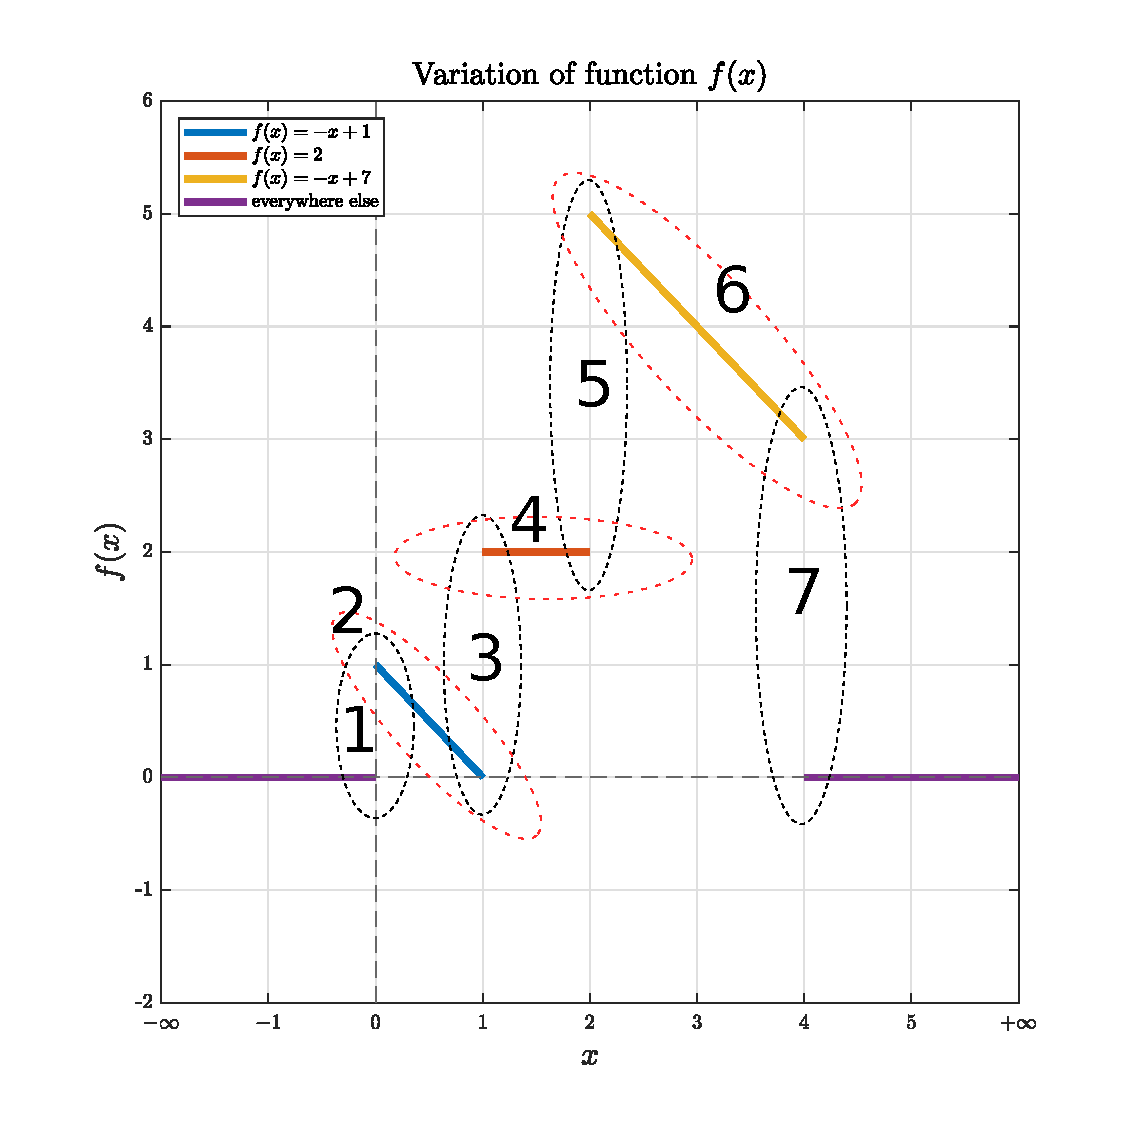
\includegraphics[width=0.7\textwidth]{totalvariation_inv.eps}
	\caption{Variation of function $f(x)$.}
	\label{\LABEL}
\end{figure}
